%
\documentclass[11pt]{thesis} % draft

\title{Algorithmic Meta-Creativity}
\author{Fania Raczinski}
\date{March 2015}

% Test

\begin{document}



% FRONT
\pagestyle{fania}


\phantomsection
% \addcontentsline{toc}{chapter}{Figures}
\pagestyle{fania}\listoffigures
\clearpage


\chapter{Hitchhiker's Guide}

\startcontents[chapters]

\vfill

\begin{alltt}\sffamily
Feeling a movement of pity,
discovered the induction coil,
cette irraisonnee induction,
and entered the opening in the wall.

Only by some recherche movement,
apres coup et sous forme d'introduction,
opening his seized manuscript,
the enemy made within the enclosure of the vineyard.

Which he had thrown off at the beginning of his labor,
in opening so exactly at the,
than the thirst of my paternity.

We can then start at once,
and whose informing voice had consigned me to the hangman,
as any person at all conversant with authorship may satisfy himself at.
\end{alltt}

\newpage

% \begin{figure}[!htbp]
% \vspace{3cm}
% \centering
%   \def\svgwidth{\textwidth}
%   \input{images/pata.pdf_tex}
% \vspace{2cm}
% \end{figure}
\begin{figure}[!htbp]
\centering
  \includegraphics[width=\textwidth]{imple.pdf}
\end{figure}

\vfill

{\sffamily 
Hello World \intro, test vlah blah dhfsdhf sdifh sohdsld hf sdfh h ghdls hg. Hello World \intro, whats up \inspi~ and helllo to you too \appa~ test,. ksjdfkj sdkjgh  ksdhg sdjfh sdjfh ksdfjhsdkfhskh kgh kjhfdg kjhgfhjfh sjueyuh tyb jjhg.
Hello World \intro, test vlah blah dhfsdhf sdifh sohdsld hf sdfh h ghdls hg. Hello World \intro, whats up \inspi~ and helllo to you too \appa~ test,. ksjdfkj sdkjgh  ksdhg sdjfh sdjfh ksdfjhsdkfhskh kgh kjhfdg kjhgfhjfh sjueyuh tyb jjhg.
Hello World \intro, test vlah blah dhfsdhf sdifh sohdsld hf sdfh h ghdls hg. Hello World \intro, whats up \inspi~ and helllo to you too \appa~ test,. ksjdfkj sdkjgh  ksdhg sdjfh sdjfh ksdfjhsdkfhskh kgh kjhfdg kjhgfhjfh sjueyuh tyb jjhg.
}

\begin{figure}[!htbp]
\centering
  \includegraphics[width=\textwidth]{legend.pdf}
\end{figure}






\newpage
% {\Large\sffamily\scshape\textbf{1.0 \quad Introduction Contents}}
% \vspace{0.5cm}
\minicontents
\spirals

\section{Thesis Map}

The following page (figure~\ref{map} on page~\pageref{map}) shows a map for this thesis, with one coloured line for each chapter and a river or lake for each appendix. This is directly modeled on the Metro map for Paris; in fact, the condensed Paris metro \autocite{ParisMetro} has 14 numbered lines (1--14) and 5 additional alphabetical lines (A--E) which correspond perfectly to the structure of my thesis.

\begin{figure}
  \centering
  \begin{tikzpicture}
  \fill[intro] (0,9.75) rectangle (1.5,10.25);
  \draw (2,10) node[anchor=west] {1. Introduction};

  \fill[inspi] (0,9) rectangle (1.5,9.5);
  \draw (2,9.25) node[anchor=west] {2. Inspirations};

  \fill[metho] (0,8.25) rectangle (1.5,8.75);
  \draw (2,8.5) node[anchor=west] {3. Methodology};

  \fill[pata] (0,7.5) rectangle (1.5,8);
  \draw (2,7.75) node[anchor=west] {4. Pataphysics};

  \fill[creat] (0,6.75) rectangle (1.5,7.25);
  \draw (2,7) node[anchor=west] {5. Creativity};

  \fill[tech] (0,6) rectangle (1.5,6.5);
  \draw (2,6.25) node[anchor=west] {6. Technology};

  \fill[eval] (0,5.25) rectangle (1.5,5.75);
  \draw (2,5.5) node[anchor=west] {7. Evaluation};

  \fill[found] (0,4.5) rectangle (1.5,5);
  \draw (2,4.75) node[anchor=west] {8. Foundations};

  \fill[inter] (0,3.75) rectangle (1.5,4.25);
  \draw (2,4) node[anchor=west] {9. Interpretation};

  \fill[imple] (0,3) rectangle (1.5,3.5);
  \draw (2,3.25) node[anchor=west] {10. Implementation};

  \fill[appli] (0,2.25) rectangle (1.5,2.75);
  \draw (2,2.5) node[anchor=west] {11. Applications};

  \fill[anal] (0,1.5) rectangle (1.5,2);
  \draw (2,1.75) node[anchor=west] {12. Patanalysis};

  \fill[aspi] (0,0.75) rectangle (1.5,1.25);
  \draw (2,1) node[anchor=west] {13. Aspirations};

  \fill[outro] (0,0) rectangle (1.5,0.5);
  \draw (2,0.25) node[anchor=west] {14. Outroduction};
  
  
  \fill[appA,opacity=0.25] (7,9.75) rectangle (8.5,10.25);
  \draw (9,10) node[anchor=west] {A. Random};
  
  \fill[appB,opacity=0.3] (7,9) rectangle (8.5,9.5);
  \draw (9,9.25) node[anchor=west] {B. Code};

  \fill[appC,opacity=0.4] (7,8.25) rectangle (8.5,8.75);
  \draw (9,8.5) node[anchor=west] {C. WordNet};

  \fill[appD,opacity=0.25] (7,7.5) rectangle (8.5,8);
  \draw (9,7.75) node[anchor=west] {D. Git History};

  \fill[appE,opacity=0.4] (7,6.75) rectangle (8.5,7.25);
  \draw (9,7) node[anchor=west] {E. Publications};
  
  
  \draw[line width=2.5pt] (7.75,5.5) circle (8.5pt);
  \draw (9,5.5) node[anchor=west] {Interchange};
  
  \filldraw[line width=2.5pt, fill=water, rotate around={45:(7.75,4.75)}] (7.5,4.5) rectangle (8,5);
  \draw (9,4.75) node[anchor=west] {Harbour};
  
  \fill[metho] (7.6,4) rectangle (8,4.2);
  \draw (9,4) node[anchor=west] {Station};


  \fill[topic] (7,2.5) rectangle (8.5,3);
  \draw (9,2.75) node[anchor=west] {Topic Cluster};
  \end{tikzpicture}
\end{figure}

There is no particular order to stations of a line, i.e. they do not correspond to the order of sections within chapters. Rather, they are more losely based on the content discussed in each chapter. Interchanges indicate where one line overlaps with another line, meaning the content discussed in the relevant chapter is related. Not all interchanges have labels --- in this case they just highlight a more general relationship. Practically, most of the stations and intersections directly represent the margin notes presented in the thesis document.

Large clusters of interchanges have been highlighted by topic clusters in light grey with appropriate labels. These clearly show the core themes covered in this thesis.

\begin{description}
  \item [Patalgorithms] This cluster contains stations related to the artefact pata.physics.wtf and the pataphysicalisation process (including the pataphysical algorithms).
  \item [Evaluation Framework] This cluster is related to the evaluation/interpretation framework developed in chapter~\ref{ch:interpretation}.
  \item [Creativity \& Computers] Here, we find stations for disciplines such as creative computing and computational creativity, but also creative search evaluation, browsing, ranking and transdisciplinarity. 
  \item [Creativity \& Pataphysics] This group contains interchanges on topics such as speculative computing and comparisons between pataphysics and creativity.
  \item [Creativity \& Intelligence] Here, we have stations on the relationship between \acs{AI}, computer ethics, and artificial creativity. Turing features heavily in this group, with his famous Turing test, and Searle with his Chinese Room.
  \item [Inspirations] This cluster mainly features the various key inspirations for this project, such as the Syzygy Surfer, Jarry's Faustroll, Borge's Chinese Encyclopaedia, and Raymond Queneau's `Cent Mille Milliards de Poèmes'.
  \item [Boden] This cluster is a reference point to the strong influence by Margaret Boden's theory of creativity on this thesis, which is used prominently in research on creative computing and computational creativity.
\end{description}

Rivers and lakes represent the appendices. 

\spirals

In addition to the map shown on page~\pageref{map} there are individual line maps at the beginning of each chapter. These show the interchanges to other lines, giving a rough overview of which other chapters relate to the content of the current chapter in one way or other. Again, this is not in order of chapter sections and subsections.

\clearpage
\begin{figure}[!htbp]
\centering
  \includegraphics[width=\linewidth]{map}
\captionsetup{textformat=empty,labelformat=blank}
\caption[Thesis Map]{Thesis Map}
\label{map}
\end{figure}

\stopcontents[chapters]

\end{document}
